\documentclass[uplatex,11pt,a4j]{jsarticle}

\usepackage[dvipdfmx]{graphicx}
\usepackage{amsmath,amssymb}

\title{LaTeXゼミ}
\author{外村 耀平}
\date{\today}
\begin{document}
\maketitle

\section{TeXについて}

\section{LaTeXのコンパイル方法}

latexmk -pvc sample.tex

\section{摘要}
\begin{abstract}
この文書ではLaTeXの書き方について説明する。ああああああああああああああああああああああああああああああああああああああああああああああああああああああああああああああああ
\\
\noindent
見出し用語:AdaBoost 分類器,網膜画像, 血管分割
\end{abstract}


\section{箇条書き}

\begin{itemize}
\item 箇条書き
\item 箇条書き
\item 箇条書き
\end{itemize}

番号付きの箇条書きを作ることをもできる.
\begin{enumerate}
\item 箇条書き
\item 箇条書き
\item 箇条書き
\end{enumerate}

\section{数式の書き方}
新しい行に改行して数式を書くことが出来る.
\begin{align}
x^2 + 2x + 1 &= 0 \\
(x + 1)^2 &= 0
\end{align}

文中に数式$x^2 + 2x + 1 = 0$を挿入することもできる.

\subsection{すこし複雑な数式}
\begin{align}
  \int_{1}^{4}x dx &= \left[ \frac{1}{2}x^2 \right]_1^4 \\
  x &= \left. \frac{2k + 1}{ \frac{2k}{k^2+5}} \right|
\end{align}

\subsection{行列式}
\begin{align}
\left(
\begin{array}{ccc}
  1 & 2 & 3 \\
  4 & 5 & 6
\end{array}
\right)
\end{align}

\subsection{注意点}
\begin{align}
\times precision &=
\displaystyle \frac{true\ positive}{true\ positive + false\ positive} \nonumber\\
\bigcirc \mathrm{recall} &=
\displaystyle \frac{ \mathrm{true\ positive}}{\mathrm{true\ positive} + \mathrm{false\ negative}} \nonumber
\end{align}

\section{図の貼り方}
\begin{figure}[htbp]
  \centering
  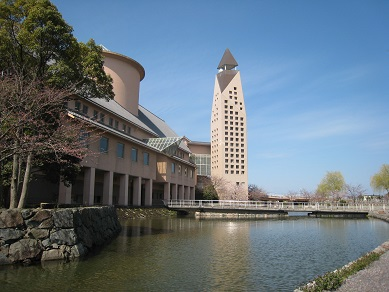
\includegraphics[width=0.5\hsize]{./figures/kendai_a22.jpg}
  \caption{figure sample}
  \label{fig:sample}
\end{figure}

\subsection{図を並べる}
\begin{figure}[htbp]
  \centering
  \begin{minipage}{0.48\hsize}
    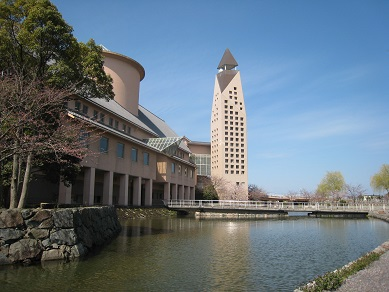
\includegraphics[width=\hsize]{./figures/kendai_a22.jpg}
  \end{minipage}
  \begin{minipage}{0.48\hsize}
    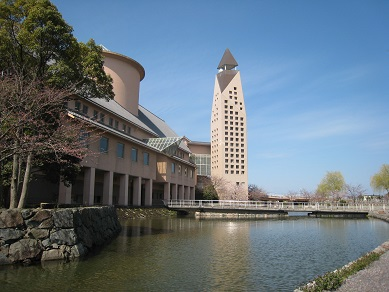
\includegraphics[width=\hsize]{./figures/kendai_a22.jpg}
  \end{minipage}
  \caption{2 figures sample}
\end{figure}

\subsection{図を並べる}
\begin{figure}[htbp]
  \centering
  \begin{minipage}{0.3\hsize}
    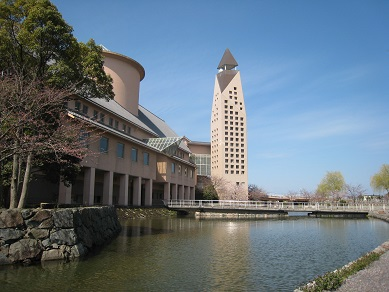
\includegraphics[width=\hsize]{./figures/kendai_a22.jpg}
  \end{minipage}
  \begin{minipage}{0.3\hsize}
    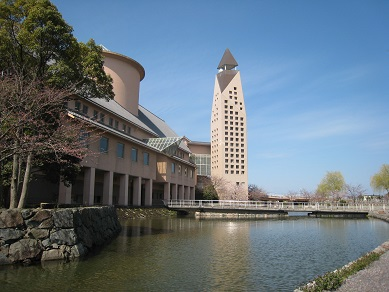
\includegraphics[width=\hsize]{./figures/kendai_a22.jpg}
  \end{minipage}
  \begin{minipage}{0.3\hsize}
    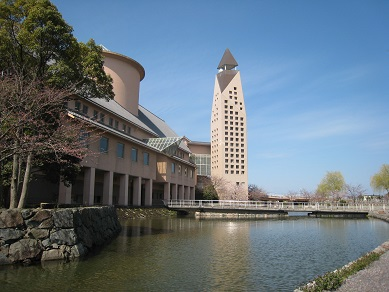
\includegraphics[width=\hsize]{./figures/kendai_a22.jpg}
  \end{minipage}
\end{figure}

\section{表の作成}
\begin{table}[htbp]
  \caption{table sample}
  \label{tb:sample}
  \centering
  \begin{tabular}{lcr}
    \hline
    番号 & 名前 & 点数 \\
    \hline \hline
    1 & 一郎 & 100 \\
    2 & 次郎 & 95 \\
    3 & 三郎 & 60 \\
    \hline
  \end{tabular}
\end{table}



\begin{thebibliography}{99}
  \bibitem{キー1} 著者:タイトル1,出典,(年)
  \bibitem{キー2} 著者:タイトル2,出典,(年)
\end{thebibliography}


\end{document}
